% Transporte paralelo en variedades
% Compilar con: pdflatex parallel_transport.tex
\documentclass[tikz,border=10pt]{standalone}
\usepackage{tikz}
\usepackage{amsmath}
\usepackage{xcolor}
\definecolor{gdlblue}{RGB}{41, 98, 168}
\definecolor{gdlred}{RGB}{191, 49, 49}
\definecolor{gdlgreen}{RGB}{30, 130, 76}
\definecolor{gdlorange}{RGB}{217, 130, 30}
\definecolor{gdlpurple}{RGB}{118, 56, 138}
\definecolor{gdlgray}{RGB}{140, 140, 140}
\definecolor{gdlyellow}{RGB}{190, 140, 10}
\usetikzlibrary{arrows.meta, decorations.markings, calc, 3d}

\begin{document}
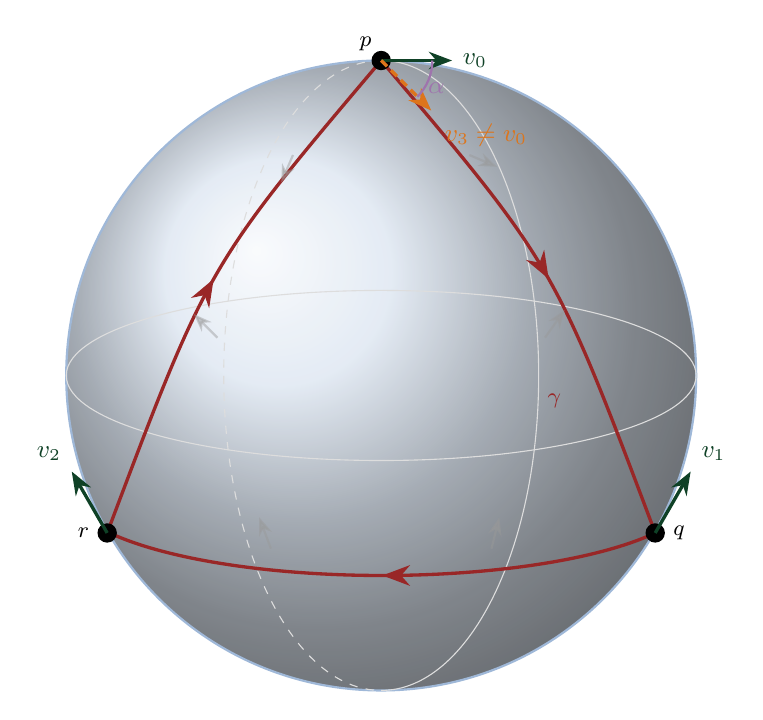
\begin{tikzpicture}[>=Stealth]

% === Parámetros ===
\def\R{4}          % Radio de la esfera
\def\ecc{0.27}     % Excentricidad elipses (perspectiva)

% === Esfera ===
\shade[ball color=gdlblue!20, opacity=0.85] (0,0) circle (\R cm);
\draw[thick, gdlblue!45] (0,0) circle (\R cm);

% Ecuador (referencia visual)
\draw[gdlgray!30] (0,0) ellipse ({\R cm} and {\R*\ecc cm});

% Meridianos sutiles
\draw[gdlgray!30] (0,-\R) arc (-90:90:{0.5*\R cm} and {\R cm});
\draw[gdlgray!30, dashed] (0,\R) arc (90:270:{0.5*\R cm} and {\R cm});

% === Vértices del triángulo esférico ===
\coordinate (P) at (0, \R);                 % Polo norte p
\coordinate (Q) at ({0.87*\R}, {-0.5*\R});  % Punto derecho
\coordinate (R) at ({-0.87*\R}, {-0.5*\R}); % Punto izquierdo

% === Curva gamma (triángulo esférico) con flechas de dirección ===
\tikzset{
    midarrow/.style={
        decoration={markings, mark=at position 0.5 with {
            \arrow[gdlred!80!black, line width=1pt]{Stealth[length=3.5mm]}}},
        postaction={decorate}
    }
}

% Lado p -> q
\draw[very thick, gdlred!80!black, midarrow]
    (P) .. controls ({0.55*\R}, {0.35*\R}) .. (Q);

% Lado q -> r (arco por el ecuador)
\draw[very thick, gdlred!80!black, midarrow]
    (Q) arc (-30:-150:{\R cm} and {\R*\ecc cm});

% Lado r -> p
\draw[very thick, gdlred!80!black, midarrow]
    (R) .. controls ({-0.55*\R}, {0.35*\R}) .. (P);

% === Puntos (negro sólido) ===
\fill[black] (P) circle (3.5pt);
\fill[black] (Q) circle (3.5pt);
\fill[black] (R) circle (3.5pt);

% Etiquetas de puntos
\node[above left, font=\footnotesize] at (P) {$p$};
\node[right=3pt, font=\footnotesize] at (Q) {$q$};
\node[left=3pt, font=\footnotesize] at (R) {$r$};

% Etiqueta de curva
\node[gdlred!80!black, font=\footnotesize] at ({0.55*\R}, {-0.08*\R}) {$\gamma$};

% === Vectores fantasma (intermedios, transporte gradual) ===
% Vectores cortos, semitransparentes, tangentes a la esfera en cada punto

% Lado p -> q: 2 fantasmas
\draw[->, thick, black!40, opacity=0.45]
    ({0.28*\R}, {0.7*\R}) -- ++({0.35}, {-0.15});
\draw[->, thick, black!40, opacity=0.45]
    ({0.52*\R}, {0.12*\R}) -- ++({0.25}, {0.35});

% Lado q -> r: 2 fantasmas
\draw[->, thick, black!40, opacity=0.45]
    ({0.35*\R}, {-0.55*\R}) -- ++({0.1}, {0.4});
\draw[->, thick, black!40, opacity=0.45]
    ({-0.35*\R}, {-0.55*\R}) -- ++({-0.15}, {0.4});

% Lado r -> p: 2 fantasmas
\draw[->, thick, black!40, opacity=0.45]
    ({-0.52*\R}, {0.12*\R}) -- ++({-0.3}, {0.3});
\draw[->, thick, black!40, opacity=0.45]
    ({-0.28*\R}, {0.7*\R}) -- ++({-0.15}, {-0.35});

% === Vectores principales transportados ===
% v_0 en p: tangente horizontal hacia la derecha
\draw[->, very thick, gdlgreen!50!black] (P) -- ++(0.9, 0)
    node[right, font=\small] {$v_0$};

% v_1 en q: tangente a la esfera, perpendicular al radio (0.87, -0.5)
\draw[->, very thick, gdlgreen!50!black] (Q) -- ++(0.45, 0.78)
    node[above right, font=\small] {$v_1$};

% v_2 en r: tangente a la esfera, perpendicular al radio (-0.87, -0.5)
\draw[->, very thick, gdlgreen!50!black] (R) -- ++(-0.45, 0.78)
    node[above left, font=\small] {$v_2$};

% v_3 en p: resultado de la holonomía (rotado 45° en sentido horario)
% Conserva fuerte componente horizontal para verse tangente al polo
\draw[->, very thick, gdlorange!90!red, densely dashed] (P) -- ++(0.636, -0.636)
    node[below right=1pt, font=\small] {$v_3 \neq v_0$};

% === Arco de holonomía alpha ===
% Arco desde v_0 (0°) hasta v_3 (-45°), sentido horario
\draw[thick, gdlpurple!70] ([shift=(0:0.65cm)] P) arc (0:-45:0.65cm);
\node[gdlpurple!70, font=\small] at (0.7, {\R - 0.35}) {$\alpha$};

\end{tikzpicture}
\end{document}
